\chapter{Testování} 		
Testování je nedílnou součástí vývoje každé aplikace. Testuje se jednak z hlediska funkčnosti a splnění požadavků, ale také z hlediska použitelnosti uživateli. Testy tedy dělíme na dvě kategorie - testy bez uživatele, neboli automatické a testy s uživatelem, tedy manuální.  Automatické testování může mít různý charakter, lze testovat funkčnost jednotlivých částí systemu, například pomocí unit testů, ale také například kvalitu kódu pomoci jeho statické analýzy. Testy s uživatelem hlavně řeší použitelnost programu, tedy zda uživatel dokáže se systémem bez problému manipulovat. Tyto testy se často provádí prostřednictvím osobního sezení, kdy uživatel dostane sadu úkolů, které má splnit a testující zapisuje, co dělalo uživateli problémy. Aby byl test smysluplný, určí se nejdříve cílová skupina, na kterou se má software zaměřovat. Určením cílové skupiny se eliminuji případy, kdy uživatel nemá dostatečné předpoklady pro užití softwaru. Pro zjištění, zda testovaný člověk do této skupiny spadá, slouží pretest dotazníky v různých formách. Bývá zvykem probrat s uživatelem po testu, například formou dotazníku, jak se mu se systémem pracovalo, jaké měl problémy, výhody a nevýhody systému, aby testující získal co nejvíce informací.  

Frameworky v této práci byly vytvořeny v první řadě jako proof of concept, což znamená, že se nejedná o verzi, ktera byla určena k vydání. Z tohoto důvodu bylo množství testů redukováno . Bylo provedeno několik ukázkových unit testů a test s uživateli na použití frameworku z hlediska vývojáře. Také byl proveden jednoduchý výkonnostní test, který zkoumá rychlost frameworku v závislosti na složitosti vytvářené komponenty.

\section{Unit testy} 
Unit testy byly pojmenovány podle toho, že testují co nejmenší části, jednotky, zdrojového kódu aplikace. Unit testy by měly testovat jednotlivé metody systému a komunikaci mezi nimi, neměly by testovat celý systém. Ideálně by každý test měl být nezávislý na ostatních testech. Výhodou unit testů je, že odhalí chyby relativně brzo v procesu vývoje aplikace. V některých případech jsou unit testy vytvářeny předtím, než vývojář začně vůbec funkcionalitu implementovat. Při vytváření testů je nutné zvážit, zda se test vůbec oplatí dělat. Obvykle se testují jen klíčové části systému, jejichž rozsah závisí na zadání a účelu systému.  

Pro testování Android frameworku byl využit testovací framework JUnit \cite{junit} a pro WP verzi byly použity testovací nástoje Visual Studia \cite{vs-unit}. Oba nástroje disponují množstvím různých porovnávání, lze určit chování testu a dalšími způsoby test přizpůsobit. V JUnit k tomuto slouží anotace, kterými lze například určit, co se vykoná před každým spuštěním testu nebo po jeho dokončení. Lze spustit jeden nebo více unit testů najednou. Vývojová prostředí většinou disponují nástrojem, který přehledně ukáže výsledky testů a případné chyby. 

V Android frameworku byly provedeny tyto testy:
\begin{itemize}
\item Test JSON parseru, který parsuje metadata přicházející ze serveru. Testuje se, zda jsou správně rozparsovány a uloženy všechny vlastnosti. Test je proveden na dvou řetězcích popisující metadata. Jeden z nich je v počádku a druhý poškozen.
\item Test utility, která parsuje z textové reprezentace datum. Metoda umí parsovat ze dvou formátů. Testují se převedení pomocí obou formátů a je také proveden test na neexistující formát, při kterém by metoda měla vrátit null.
\item Test správného vytvoření adresy z definovaného připojení. Testuje se případ s portem a bez portu.
\end{itemize} 
Ve Windows Phone verzi byly provedeny následující testy:
\begin{itemize}
\item Stejné testy jako v případě Androidu.
\item Test nahrazení proměnných v XML souboru se zdroji hodnotami z Dictionary. Tyto hodnoty mohou ovlivňovat, jak je zdroj nadefinován a tedy i proces připojení na něj. Tento test hlavně testuje správné přepsání z Javy do C\#, protože Java metoda již byla otestována \cite{tomasek-thesis}.
\item Test na získání výčtového typu podle jeho hodnoty. V C\# nejsou totiž stejné výštové typy jako v Javě a nelze jim jednoduše nadefinovat hodnotu. Výčtové typy ve WP verzi se snaží přiblížit chování Java enumů a s tím souvisí i metoda valueOf, která by na základě hodnoty měla vrátit příslušný výčtový typ. Tento test ověřuje její správnost.
\end{itemize} 

\section{Test s uživatelem}
Při návrhu frameworků bylo potřeba zaměřit se hlavně na potřeby vývojářů mobilních aplikací. Každý takový vývojář je už zvyklý na určité možnosti a vlastnosti, které při vývoji používá. Například by měl framework umožnit nastavovat vzhled komponent. Při návrhu testu jsem čerpal z předmětu Testování uživatelských rozhraní, kde jsem podobný test navrhoval v rámci semestrální úlohy. Bylo třeba určit cílovou skupinu a navrhnout úkoly pro test. Také bylo žádoucí získat od partipantů další informace, například jaký mají z frameworku dojem.

\subsection{Cílová skupina}
Cílovou skupinou pro tento test jsou výjojáři Android nebo Windows Phone aplikací. Účastníci testu by měly vědět jak vytvořit layout, do kterého by mohly frameworkem vytvářené komponenty vkládat, umět si vytvořit tlačítko, na které naváží například odeslání formuláře. Zkušenosti vývojáře se standartním vývojem mobilních aplikací jsou důležité i proto, aby byl schopen porovnat přístup frameworku s klasickým způsobem. Potencionální účastníci testu byli vybírání z mého ročníku a byli kontaktováni osobně či skrz sociální sítě. Bylo osloveno celkem deset lidí, o kterých jsem předpokládal potřebné zkušenosti, z nichž tři lidé požadavky nesplňovali a dva lidé test odmítli. Ze zbývajících pěti lidí uměli tři Android a dva Windows Phone. Pro vyváženost testu byl jeden participant, který uměl Android odmítnut.    

\subsection{Příprava testu}	
Pro test byla vytvořena sada úkolů a uživatelská příručka. Aby nebyl test příliš časově náročný, byla příručka rozeslána participantům předem s tím, že mohou mít ke všemu dotazy. Participanti měli vytvořit novou klientskou aplikaci nebo použít existující, do které si sami lokálně naimportují příslušný framework. K tomu bylo nutné jim framework poskytnout. Participanti pro test nepotřebovali v podstatě nic. Vlastní telefon s Androidem nebo WindowsPhonem a naisntalované IDE pro vývoj bylo výhodou. Vyvíjet však mohli i na mém notebooku, kde bylo pro participanty připraveno VisualStudio 2015 a AndroidStudio 1.5.1. K odzkoušení aplikací byly připraveny smartphony s Androidem 4.3 nebo Windows Phone 8.1. V případě Androidu bylo možno využít také emulátor obsahující Android 6.0. K testu byla potřeba serverová část
 
\subsection{Testované úkoly}
Testované úkoly byly navrženy tak, aby pokryly co největší množství frameworkem poskytované funkcionality a pokud možno na sebe navazovaly. V úvahu byla vzata i náročnost úkolů. Po dokončení většiny úkolů se předpokládalo, že si participant aplikaci nahraje do zařízení a odzkouší ji. Pokud tak uživatel neučinil, bylo mu to připomenuto. K programování mohl testovaný používat přiloženou uživatelskou příručku. Časová náročnost testu bylo odhadnuta na zhruba jednu hodinu a patnáct minut. Uživateli byly testované úkoly předány ve formě PDF souboru v následujícím pořadí.

\begin{enumerate}
\item Před testem prostudujte uživatelskou příručku, pokud jste již tak neučinili.
\item Založte si novou aplikaci nebo si otevřete existující a importujte do ní framework.
\item Vytvořte si XML soubor pro definici připojení. V něm vytvořte dvě připojení pro formulář a list, které si libovolně pojmenujte. 
\begin{enumerate}
\item Formulář
\begin{enumerate}
\item Definice komponenty je na adrese \url{http://toms-cz.com/AFServer/rest/country/definition}. Zdroj je veřejný a poskytuje data ve formátu JSON.
\item Formulář lze odeslat na adresu \url{http://toms-cz.com/AFServer/rest/country}. Zdroj je zabezpečený, může k němu přistupovat jen přihlášený uživatel. Server očekává data ve formátu JSON.
\end{enumerate}
\item List
\begin{enumerate}
\item Definice komponenty je na adrese \url{http://toms-cz.com/AFServer/rest/country/definition}. Zdroj je veřejný a poskytuje data ve formátu JSON.
\item Data, kterými lze list naplnit jsou na adrese \url{http://toms-cz.com/AFServer/rest/country/list}.  Zdroj je veřejný a poskytuje data ve formátu JSON.
\end{enumerate}
\end{enumerate}
\item Vytvořte prázdný formulář přidávající/upravující zemi a libovolně ho vložte do aplikace. Komponentu vhodně pojmenujte.
\item Vytvořte list naplněný existujícími zeměmi. Komponentu vhodně pojmenujte.
\item Zajistěte jazykovou srozumitelnost komponent (tj. v češtině nebo angličtině).
\item Zprovozněte odesílání formuláře po stisknutí vámi vytvořeného tlačítko.
\begin{enumerate}
\item Posluchač události vytvořte nejlépe ve zvláštní metodě.
\item Po odeslání informujte uživatele o úspěchu/neúspěchu akce.
\item Volitelně zprovozněte reset a clear formuláře.
\end{enumerate}
\item Upravte libovolně vzhled formuláře (např. změňte barvu labelů)
\item Upravte libovolně vzhled listu (například upravte border listu)
\item Propojte list s formulářem tak, že po kliknutí na položku listu se data nahrají do formuláře
\end{enumerate}
\subsection{Výsledky testu}
Všichni testovaní zvládli splinit všechny úkoly zhruba v odhadovaném časovém limitu bez větších komplikací. Nicméně někdy bylo potřeba testovanému trochu poradit. Nejzávažnějším problémem pro testované bylo pochopit, jak funguje a k čemu přesně slouží XML soubor pro definici připojení. Většina testovaných postupovala podle uživatelské příručky, kde se nalézá ukázkový kód pro definici všech tří zdrojů a tento kód zkopírovala a dále upravovala. Nejvíce uživatele zarazilo, když měl být zdroj veřejný, tedy nebyl nijak zabezpečený a pouze nebylo třeba definovat dodatečné bezpečnostní parametry v uzlu <security-params>, uživatelé však chtěli tuto skutečnost někde nadefinovat a strávili dlouhou chvíli hledáním v příručce. Dva participanti si jednotlivá připojení libovolně pojmenovali, tedy nastavili připojení vlastní identifikátor, dva zanechali identifikátor ze zkopírovaného kódu z příručky, ale v průběhu testu jim skutečnost, že id nezměnili, došla. Zabrat daly uživatelům také hodnoty určené k nahrazení v XML souboru, uživatelé pochopili, že se budou hodnoty získávat z mapy nebo slovníku, který je předáván jako poslední parametr metody na inicializaci builderu, ale už jim nedošlo, kde mají mapu či slovník vzít. Jelikož je v uživatelské příručce zobrazena ukázka kódu z ukázkového projektu, kde je tato mapa či slovník získávána skrz utils metodu. Uživatelé chtěli tuto metodu použít a byli trochu překvapeni, když ji nemohli nalézt. Po krátkém vysvětlení, že se v ukázkové části kódu jedná o výtržek z ukázkové aplikace, už bylo všem jasné, že si musí mapu či slovník vytvořit sami. Někteří ještě chvíli tápali, jaké hodnoty do mapy vložit, zkoušeli jako klíč uživatelské jméno a hodnotu heslo, ale nakonec všem správné použití došlo samovolně bez jakékoliv pomoci. Obrázek jedné z aplikcí vytvořených v rámci testování je zobrazen v příloze \ref{img:testApp}.

Uživatelé na framework reagovali kladně. V průběhu testu se o něj zajímali a vnímají ho jako silný nástroj. Samozřejmě byly i připomínky. Windows Phone uživatelé moc dobře poznali, že je WP verze přepisována z Javy a vnímali WP framework jako příliš javovský, což nepokládali za překážku, ale spíše jako estetiskou vadu. Testovaní také měli pocit, že některé části by mohly být lépe zdokumentovany v uživatelské příručce. Jejich výtky jsem si zapisoval a v uživatelské příručce později změnil. Seznam všech problému a návrhů jejich řešení je v tabulce \ref{table:testIssues}.

\begin{table}[h!]
\begin{center}
\caption{Problémy zjištěné během testování s uživatelem}
\label{table:testIssues}
\begin{tabular}{|p{7cm}|p{7cm}|}
\hline
\textbf{Problém} & \textbf{Navrhované řešení} \\
\hline
Uživatelům trvalo, než pochopili smysl XML souboru pro nadefinování zdrojů. Tři ze čtyř potřebovali poradit. & Lépe popsat tuto část v uživatelské příručce. \\
\hline
Lokalizace textů na klientské straně ruší výhodu, že formulář pružně reaguje na změnu datového modelu na serveru a není tudíž potřeba vydat novou verzi aplikace. Tato verze bude muset být vydána stejně kvůli lokalizačnímu textu. & Klient bude při získání zdroje posílat jazyk a lokalizace bude provedena už na serveru a klient přijme rovnou konkrétní překlad. \\
\hline
Získání dat z položky v listu chtěl uživatel provádět manuálně, tedy získat data z položky ve formě mapy a poté nastavovat data jednotlivým polím, i když na to existuje metoda. & Lze použít metodu, která získá správnou reprezentaci dat pro naplnění formuláře skrz metodu insertData, která se používá i při plnění daty ze serveru. Lépe tento fakt zdokumentovat v uživatelské příručce. \\
\hline
List disponuje metodou getView, která získá jeho celkovou grafickou reprezentaci, ale také metodou getListView, která slouží k získání pouze její části, existuje však, aby šlo na tuto část připojit posluchač událostí. Uživatelé nevěděli, kterou metodu využít pro získání UI reprezentace, kterou mají vložit. & Zvážit zvolení jiných názvů metod, které by více vypovídaly o tom, k čemu metody slouží. Také lépe zdokumentovat tuto část v uživatelské příručce. \\
\hline
\end{tabular}
\end{center}
\end{table}

\section{Výkonnostní test} 
Tento test ukazuje závislost doby vytvoření komponenty na počtu částí, ze kterých se skládá a na rychlosti připojení k internetu. Test byl proveden na obou platformách. Bohužel nemůžeme platformy jednoduše mezi sebou porovnat, neboť zařízení, na kterých test proběhl, nemají stejné parametry, které taky rychlost vytváření ovlivňují. Nicméně bylo provedeno měření pro dva formuláře, jeden z nich se skládal ze dvou polí a nebyl naplněn daty, druhý měl polí čtrnáct a daty naplněn byl. Potom byl test proveden pro listy, kde bylo sledováno zda rychlost vytvoření komponenty ovlivňuje i množství dat, kterými se komponenta naplní. Jedna položka listu obsahovala u obou listů stejný počet informací, v obou listech byl ale rozdílný počet záznamů. Pro každou komponentu bylo provedeno 10 měření, ze kterých se udělal průměr. 

Test na Android platformě ukázal, že na počtu polí ve formuláři i na rychlosti připojení záleží. Zatímco menší formulář byl na Wi-Fi v průměru vytvořen za 684 milisekund, větší formulář v průměru za 1084 milisekund a potom se ještě dalších 645 ms naplňovat daty. Na mobilních datech vytvoření menšího formuláře trvalo téměř dvakrát déle, tedy 1110 milisekund, vytvoření většího trvalo přibližně 2035 milisekund bez naplnění daty a 2990 milisekund s vloženými daty. Test tvorby listu ukázal, že na množství položek v listu také záleží. List s jednou položkou se vytvořil a naplnil daty na Wi-Fi v průměru za 1450 milisekund a listu s osmi záznamy to trvalo v průměru pouze od 20 milisekund déle. Při slabším připojení byl rozdíl už markantnější, činil v průměru asi 350 milisekund.

Windows phone platforma měla hodnoty samozřejmě jiné, podstatné však je, že se chovala obdobně jako Android. Ukázalo se tedy, že záleží jednak na rychlosti připojení k internetu, počtu částí, ze kterých je komponenta vytvořena a i na množství dat, kterými je komponenta naplněna.

\section{Ukázkové projekty}
Pro otestování frameworků v praxi byly vytvořeny dva ukázkové projekty, pro každou platformu jeden. Vše, co bylo potřeba pro vytvoření klientské aplikace, byl příslušný framework a již naimplementovaná serverová strana, která byla využita i pro demonstraci AFSwinx a AFRest \cite{tomasek-thesis}. Aplikace na serveru slouží jako systém k zadávání absencí, která disponuje zdroji, ze kterých lze získat definici UI a data. Také poskytuje zdroje pro odesílání formulářů, které vytváří nebo upravují záznamy v databázi. Část zdrojů je zabezpečená a může k ní přistupovat jen uživatel s určitou rolí. Z tohoto důvodu musí v klientských aplikacích existovat security context, ve kterém je přihlášený uživatel udržován a v případě potřeby zasílán na server. 

Uživatelské rozhraní klientských aplikací umožňuje uživateli vytvořit absenci, která čeká na schválení. Uživatel s příslušnými právy ji může přijmout nebo zamítnout, svou absenci může uživatel zrušit. Typy absencí lze vytvářet a upravovat. K dispozici je také vytváření a úprava zemí. Pro každou zemi jsou typy absencí různé a tedy každý uživatel v závislosti na tom, z jaké pochází země, vidí různé druhy absencí, které může vytvořit. Také si lze zobrazit a upravit svůj uživatelský profil.

Na obrázcích, které zobrazují klientské aplikace je vždy vlevo ukázková aplikace pro Android a vpravo pro Windows Phone.

\subsection{Přihlášení}
Pro vstup do ukázkových aplikací je nejprve třeba se přihlásit. Při spuštění aplikace je zobrazen přihlašovací formulář, který lze nalézt na obrázku \ref{img:login}. Po přihlášení je uživatel uložen do aplikačního kontextu, ze kterého ho lze v případě potřeby získat. Pro přihlášení lze použít dva uživatele, kteří jsou registrování v databázi na serveru. Jeden z uživatelů má roli admina a může provádět věškeré operace. Druhý je pouhým uživatelem, což má za následek to, že se mu zobrazuje jen určitá podmnožina dat, některé aktivní prvky jsou pro něj vypnuty nebo nemá právo na odeslání formuláře.

\begin{figure}[h!]
\centering
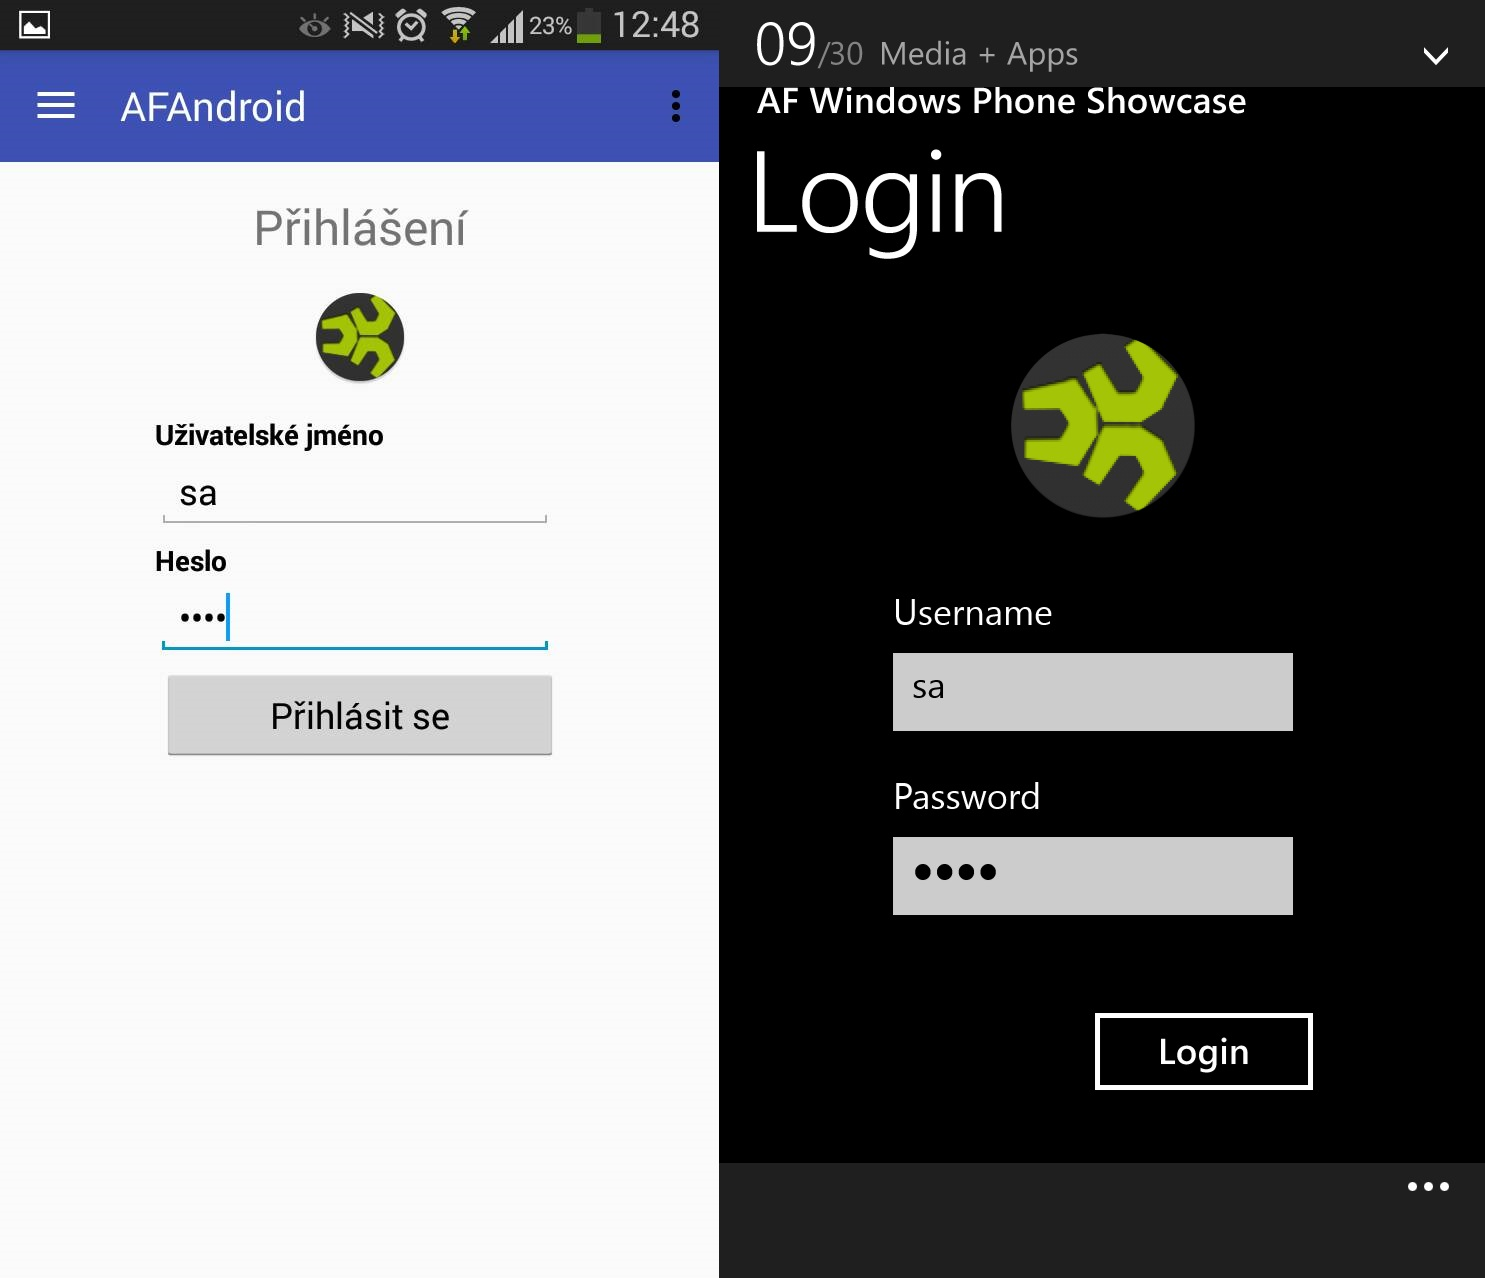
\includegraphics[width=0.5\linewidth]{figures/screenshots/Login}
\caption{Ukázkové projekty - přihlášení}  
\label{img:login}
\end{figure}

\subsection{Správa zemí}
Tato sekce obsahuje list, který zobrazuje již existující země a formulář, kterým země lze vytvořit nebo upravit, což reprezentuje obrázek \ref{img:country}. Pro upravení existující země stačí na zemi kliknout a zobrazí se její náhled ve formuláři níže. Pokud je takto formulář naplněn, tak jeho změna zemi ve formuláři edituje, pokud je formulář prázdný je provedením změn vytvořena země nová. Upravovat a přidávat země smí jen admin, obyčejný uživatel má prvky formuláře neaktivní. V případě, že by došlo k chybě a obyčejný uživatel by přesto poslal data na server, kontroluje se uživatelská role i na serveru. Po přidání či úpravě země se uživateli zobrazí výsledek akce v Androidu formou Toast zprávy, ve WP formou dialogu. Obrazovka disponuje také tlačítky na resetovaní a vyčištění formuláře.
\subsection{Správa absencí}
Dalším případem, kdy zavisí na uživatelské roli je obrazovka reprezentující správu absencí. V této sekci je pro zobrazení absencí vytvořen list a pod ním je umístěn formulář, do kterého lze nahrát data z listu a případně je upravit. Každá uživatelská role vidí v listu různá data, obyčejný uživatel vidí pouze své vytvořené absence a má možnost je zrušit či nechat ve stavu, kdy žádá o schválení, což je zobrazeno na obrázku \ref{img:AbsenceManagement}. Adminstrátor vidí všechny absence včetně svých a může je schvalovat, rušit nebo zamítnout, což je patrné z obrázku \ref{img:AbsenceManagementAdmin} . V případě, že admin žádost schválí nebo zamítne, mizí běžnému uživateli absence z listu a již s ní nelze operovat, administrátor vidí absence ve všechy čtyřech stavech. 
\subsection{Správa absenčních typů}
Každá země má své typy absencí, které lze použít. Uživatel má na výběr z typů absencí, které přísluší zemi, která je uživateli nastavena. Data v listu, který je na obrazovce se správou typů, jsou závislé na volbě země, která je reprezentována formulářem o jednom prvku, ze kterého se předá pro tvorbu listu identifikátor vybrané země. Tento formulář je v Android aplikaci ve vrchní části obrazovky. Ve Windows Phone verzi byl zvolen jiný přístup, při pokusu přejít na tuto obrazovku je nejprve zobrazen dialog s formulářem, pro výběr země. Po vybrání země a potvrzení se zobrazí již příslušný list. Formulář, který je v Android aplikaci pod listem je ve WP verzi na vedlejší stránce. Při kliku na položku v listu aplikace přejde sama na vedlejší stránku s naplněných formulářem, při úspěšném přidání či úpravě přejde aplikace z formuláře zpět na list. Tento přístup byl zvolen pro demostraci toho, že vytvořené komponenty lze opravdu vložit do jakéhokoliv jiného prvku uživatelského rozhraní. Příslušná část aplikace je zobrazena na obrázku \ref{img:AbsenceType}.
\subsection{Uživatelský profil}
Každý uživatel má svůj profil, který může v aplikaci upravovat. Tato obrazovka slouží hlavně k demostraci většiny typů aktivních prvků, které umí framework interpretovat. Pole ve formuláři upravující profil také podléhají validacím. Obrázek \ref{img:profileValidations} zobrazuje dvě z nich, validaci pravidel REQUIRED a MAX z tabulky \ref{table:validations}. Také je patrné, že je Android aplikace převážně v češtině a WP verze v angličtině, za což je zodpovědná lokalizační část frameworku. Ne všechny popisky však ze serveru přichází ve formě klíčů k přeložení a nejsou proto lokalizovány. 
